%------------------------------------%
% Début Partie Azarias				%
%------------------------------------%
\part{System design}

\chapter{User interface design}
Because the project was created with Qt, and Qt adapt its interface depending on the OS it's running on, there is no 'global' user interface. However, the layout is always the same and so is the content. The following screenshots will show the user interface as it is on Linux, more precisely Ubuntu. Currently, QTypingTest is available on Ubuntu and windows.\\
When the user starts the software, he's directly directed on the homepage, figure \ref{homepage-logout} where he can either create a new profile or connect himself to his own existing profile. The buttons allowing to go through the differents part of the software are disabled as long as no one is connected. A list of the existing user is displayed and the user just has to click on his alias to be considered as connected(figure \ref{homepage-login}. He can then go through the differents part of the user interface. 
\begin{figure}[H]
  \centering
  \begin{minipage}[b]{0.45\textwidth}
    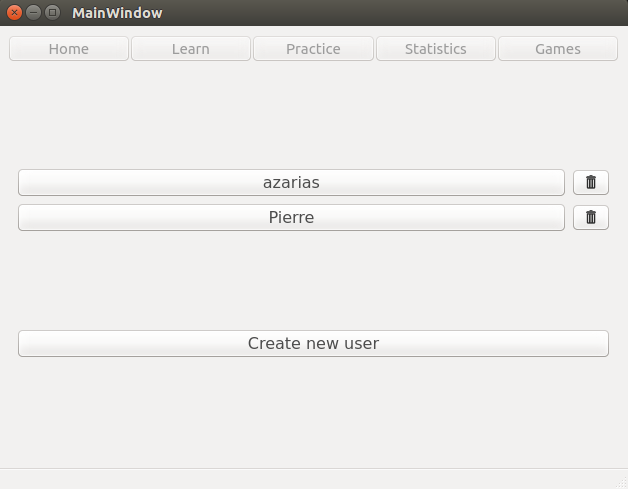
\includegraphics[width=\textwidth]{images/homepage_logout.png}
    \caption{Defaults homepage.}
    \label{homepage-logout}
  \end{minipage}
  \hfill
  \begin{minipage}[b]{0.45\textwidth}
    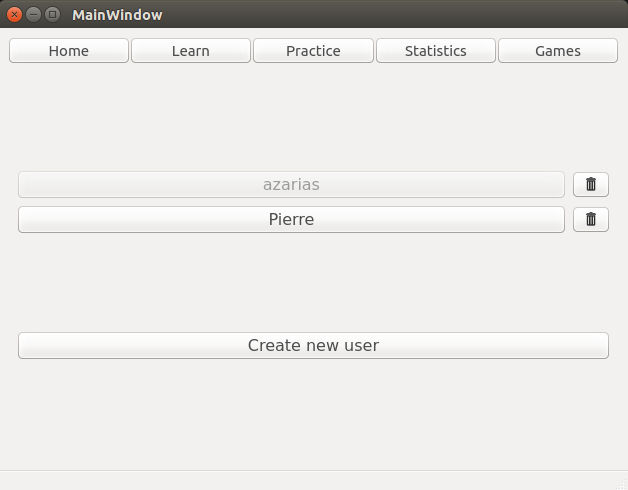
\includegraphics[width=\textwidth]{images/homepage_login.png}
    \caption{User connected.}
    \label{homepage-login}
  \end{minipage}
\end{figure}
A user can also delete his profile by clicking on the trash icon. \\
The purpose of the login system was not to be secured. Since this software is made for private use, and that it does not contain any sensible informations, the group decided to focus on the software itself and to do not spend to much time on the login system. \\
On the top of the window, there are five buttons.
\begin{itemize}
	\item Home. This button, when triggered, shows the homepage, but does not disconnect the user.
	\item Learn. This show the main part of the project. The page where the user has a list of the differents letters to learn in an certain order.
	\item Practice. On this page, the user can choose differents mode of practice.
	\item Statistics. Here, the user can see his statics.
	\item Games. Some simple games developed to learn the fun way to type.
\end{itemize}


\begin{figure}[H]
	\centering
	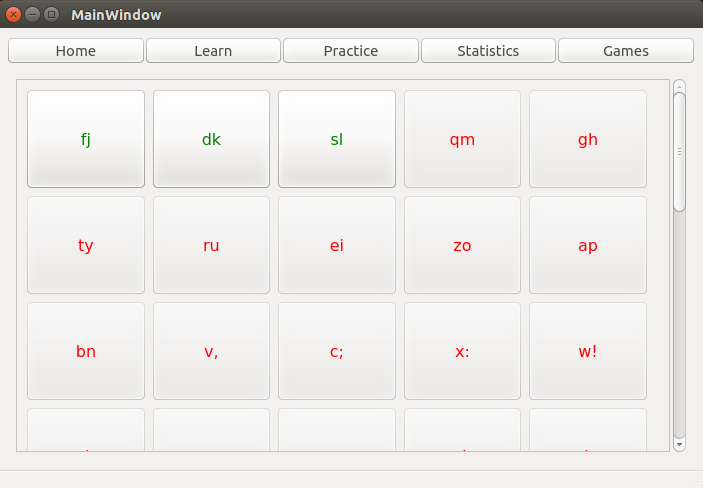
\includegraphics[width=0.7\textwidth]{images/page-learn.png}
	\caption{Learn page}
	\label{page-learn}
\end{figure}

The learn page (figure \ref{page-learn}) the user can see all the exercises to come. He must succeed to them one by one. And should realize a minimum score the be able to unlock the next exercise. When clicking on a button, a dialog is shown and the user can start a new exercise.

\begin{figure}[H]
	\centering
	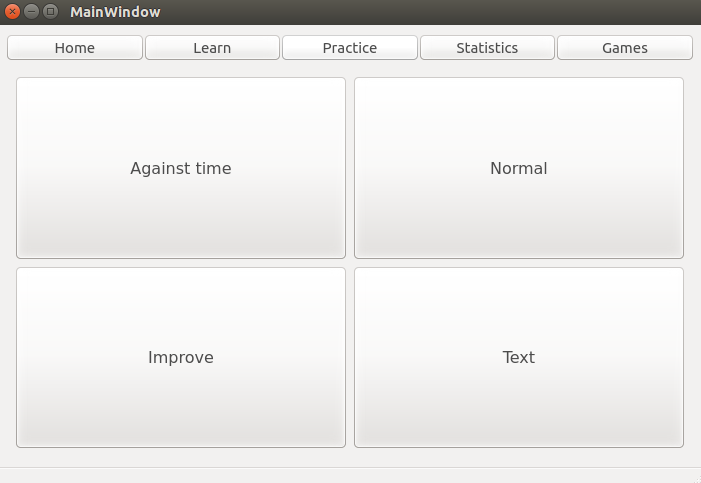
\includegraphics[width=0.7\textwidth]{images/page-practice.png}
	 \caption{Practice page}
	 \label{page-practice}
\end{figure}

The practice page  (figure \ref{page-practice}) has four buttons. One for each differents type of practice. The final 'form' of each practice is always the same : a dialog with text to type. What's changing is the content of the dialog.\\
The differents rules for each types of practice are 
\begin{description}[align=left]
	\item[Against time :] The user must type the most words in one minute. At the end of this time, his number of words per minute is shown.
	\item[Normal :] The user has two 'pages' of random words to type. Thanks to the powerful language system of Qt, the displayed words may change depending on the user's computer language. For the moment, only english and french is supporter.
	\item[Improve :] This practice will check what is the user's worst letters and create a special exercise containing these letters.
	\item[Text :] In this practice, the user will have to type an existing text. The chosen text are the 'classical' authors such as George Orwell. Once again thanks to Qt, the language of the text may vary depending on the user's computer language. The default language being english. 
\end{description}

\textit{The statistics page was not made yet}

\begin{figure}[H]
	\centering
	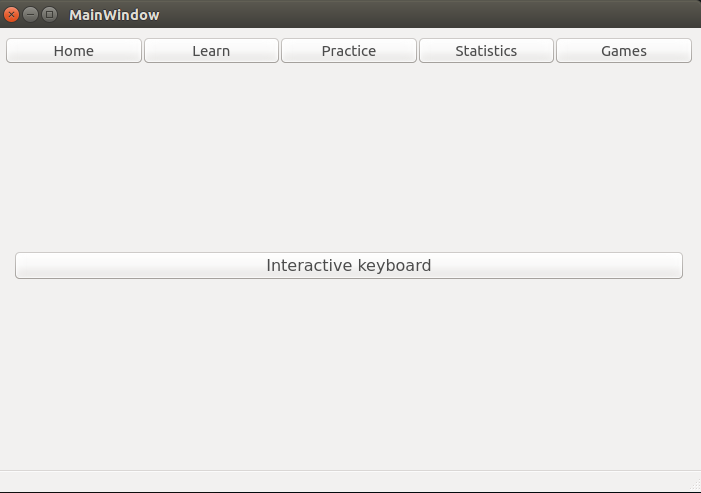
\includegraphics[width=0.7\textwidth]{images/page-games.png}
	 \caption{Game page}
	 \label{page-game}
\end{figure}

The game page contains a single button. This button launches a dialog where the user sees what letters is associated with what finger on the keyboard.

\subsection{The differents dialogs}
Here are the dialogs that can be opened with Qt :

\begin{figure}[H]
	\centering
	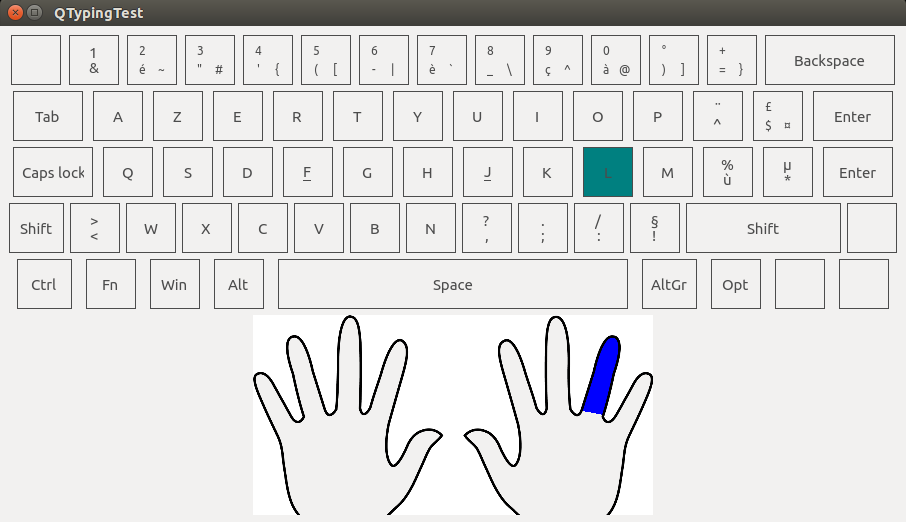
\includegraphics[width=0.7\textwidth]{images/dialog-before-learn.png}
	 \caption{Before the learning dialog}
	 \label{dialog-before-learn}
\end{figure}

Here is the dialog shown when the user starts an exercise to learn new letters.\\
This dialog highlights in a certain color the finger and associated with the letter on the keyboard. This invites the user to do the same. Thus use the indicated finger to type on the indicated letter. When he does this, the next letter and the next finger highlights. When those two steps are completed, the user can start the real exercise.\\
The pictures shows the configuration of an AZERTY keyboard, because the test are made on a french computer. But a configuration file is also made for QWERTY keyboard, and anyone who uses a non-french computer's configuration will automatically have the QWERTY configuration loaded.

\begin{figure}[H]
	\centering
	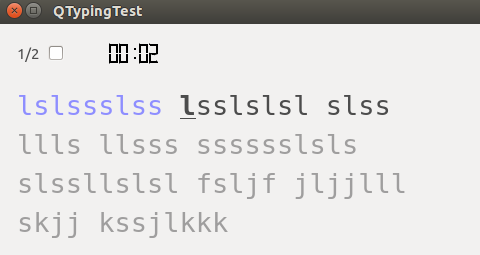
\includegraphics[width=0.7\textwidth]{images/dialog-learn.png}
	 \caption{The learning dialog}
	 \label{dialog-learn}
\end{figure}

The figure \ref{dialog-learn} shows the dialog to learn new letters. In this case, the letters are \textit{S} and \textit{L}.\\
There are two parts on the dialog : the toolbar and the center part.\\
The toolbar contains :
\begin{itemize}
	\item The page indicators that tells on what page is located the user and how many remains.
	\item The play/pause button as the check-box button. When it's toggled the game is paused and when it is not (the default) the game goes on.
	\item The timer. This tells the user how much time was spent since the start of the exercise.
\end{itemize}

The center part contains the user's exercise. It displays a text on two pages with four color codes :
\begin{itemize}
	\item Black : a normal black letter is a letter to be typed in the future
	\item Black underlined and bold : the current letter that the user has to type
	\item Blue : a letter already typed by the user and correctly typed
	\item Red  : a letter already typed by the user but incorrectly typed
\end{itemize}

The center part does not takes care of the words. It's only taking care of each letters.\\
The user can rewind back to retype the letters. This will also work from one line to another. However this is voluntary not possible
from one page to another.\\
This dialog will always look the same for the trainings and the exercise. The only difference lives in the content of the main part.\\
For the exercise dialog, the exercise is organized as so :
\begin{enumerate}
	\item For two lines, only the two letters that the user must learn.
	\item For two lines all the letters previously learned in a random order
	\item And the remain part is some random words with the letters previously learned. If no words can be made with the letters learned (especially true at the beginning) the second part will be repeated.
\end{enumerate}

\begin{figure}[H]
	\centering
	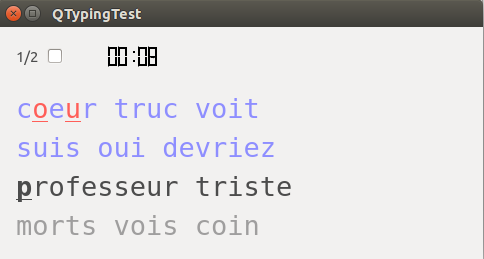
\includegraphics[width=0.7\textwidth]{images/dialog-practice.png}
	 \caption{The practice dialog}
	 \label{dialog-practice}
\end{figure}

This dialog is very similar to the learning dialog. The toolbar is exactly the same and works the same way.\\
The only difference is the content. This dialog contains only real words. In this case, it's only french words since there is a words file for french computers. There is also a file containing english words. And this file is the default one.\\
This type of exercise contains only words placed in a random order, on two pages.

\begin{figure}[H]
	\centering
	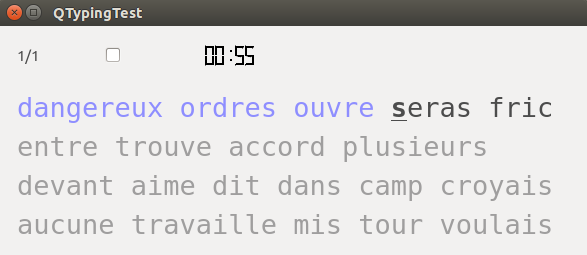
\includegraphics[width=0.7\textwidth]{images/dialog-race.png}
	 \caption{The race dialog}
	 \label{dialog-race}
\end{figure}

The race dialog is similar to the two previous one. However there is one difference in the toolbar. Instead of starting at 0, the timer starts at 1 minute, and decreases. This changes results in another change : the number of pages. Since the number of page depend on the speed of the user. It is 'unknown'. But instead of hiding this information, it will simply increase for each new page created.\\
For this exercise, only one page is generated and if the user succeed to finish the page, another one is generated and displayed. Thanks to the speed of C++ and the algorithms, the user does not see the difference. This system allows the exercise to generate (in theory) an infinite number of pages and therefore change the start time.
The content is the same as the practice dialog : it contains only words of french or english depending on the user's computer (in this case, french).\\

\begin{figure}[H]
	\centering
	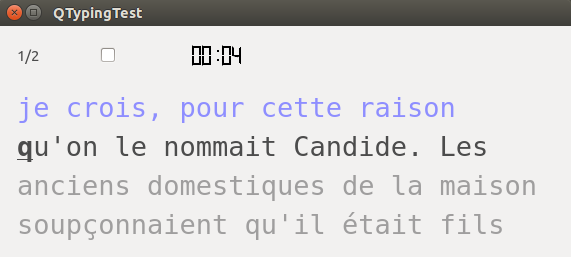
\includegraphics[width=0.7\textwidth]{images/dialog-text.png}
	 \caption{The text dialog}
	 \label{dialog-text}
\end{figure}

The text dialog is exactly the same as the practice dialog. The only difference is the content. Instead of containing only random words, it contains a real text. The text is either in french or english, depending on the user's computer configuration.

\begin{figure}[H]
	\centering
	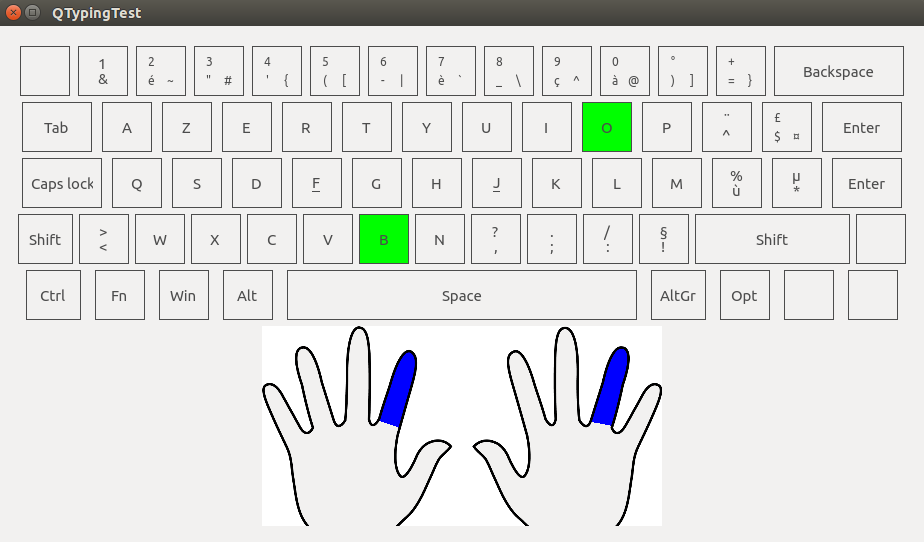
\includegraphics[width=0.7\textwidth]{images/dialog-game.png}
	 \caption{The game dialog}
	 \label{dialog-game}
\end{figure}

The game dialog is the same as the one shown before the learning exercise. But instead of showing the user what letter he has to type, it will simply let him free to type whatever letters he wants, and shows what finger is associated with this letter. \\




\section{Qt features}

Qt is a really powerful framework full of features. There are so many of them that is sometimes possible to miss one and redo all the work. That's what happened for the group many times during the development of the software.\\
Qt is first made to create user interfaces on great variety of OS. With the same source code, it is possible to have a interface for linux, windows and mac OS. But there are a lots of useful features to improve the life of the developer and some tools to improve the C++ language.\\
The most powerful feature by far of Qt is it's SIGNAL-SLOT system.

\begin{figure}[H]
	\centering
	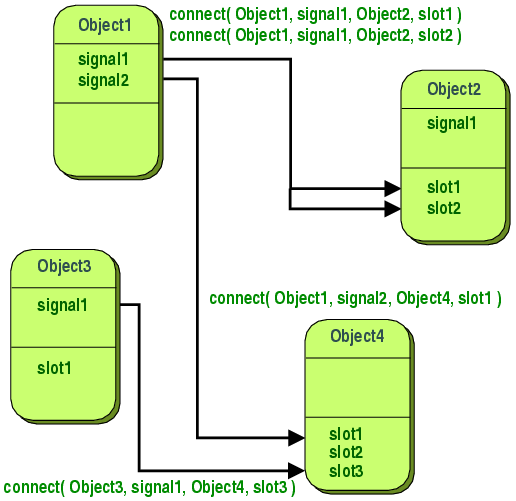
\includegraphics[width=0.7\textwidth]{images/abstract-connections.png}
	 \caption{The connection system in Qt}
	 \label{signal-slot-qt}
\end{figure}

The figure \ref{signal-slot-qt} shows how it works.
A signal can be emitted and a slot can be called whenever a signal is emitted. This is very useful to program interactive user interfaces.\\
It would be too long to enumerates all the features that Qt provides, and a lots of them where not used in the project. However, here is a list of features used for the project provided by Qt.

\begin{description}[align=left]
	\item[Language detection] : Qt can easily detect the user's computer language. This was first used to select the files for the exercises.
	\item[Resources files] : The group discovered later than Qt can actually automatically select the good file depending on the computer language. This is made thanks to a resource file (.qrc). This file is written in XML and tells Qt where to find the resource file, give them a language and give them an alias. Then, when needing a file in the code the alias of the file is given, and Qt will choose the good file depending on the computer's language.
	\item[DataStream] : It is possible with Qt to open and read or write in a file. This 	was first used to save the users in binary files. The files can also be opened in text mode to read and write UTF8-only characters. This was used to read the keyboard configuration files.
	\item[Qt Variant and metatypes] : as for the language detection, the group discovered later that Qt has a pre-made data-saving system. This provides a safer way to save the data on the computer. Instead of writing on a file in the folder of the project itself, Qt will choose a system folder depending on the OS of the computer to write down the data to save.
	\item[Json] : Qt supports the JSON format. It can parse any valid json file and be used later on in the code. This is what's actually used to save the keyboard configurations. 
	\item[XML] : As for the JSON, Qt also support XML. It can parse any XML file and return an object that can be manipulated easily. This features could have been used to save the texts.
	\item[QString] : Last be not least. Qt provides a really powerful class : the QString. This class is really easy to use, and full of functions.
\end{description}

\subsection{Documentation}
It is not a part of Qt itself, but without it, the development of the software would be impossible.\\
The documentation of Qt is available online, but also on QtCreator. It is really well-made. Easy to read comprehensive, completed with examples and consistent.\\
Moreover, when there is a problem with Qt and that the documentation cannot solve the problem, the community behind Qt is huge and really helpful.  

\chapter{Functional Design}
This project is relatively simple an contains two main parts :
\begin{description}
	\item[The learning] : where the user learn each letters of the keyboard one by one
	\item[The practising] : where the user can see the progress made by typing real words, and real texts
\end{description}
Since this software is quite simple, everyone with a computer can use it. This means the software is made for all ages. Anyone whether there are young, can use the software without a lot of explanation and learn, step by step how to correctly use his keyboard.\\
Also, thanks to Qt robustness and features, the software is viable and is unlikely to crash during its usage.

\section{Structure of the system}

\begin{itemize}
	\item The Data part. This part is where all the objects containing data are stored. e.g the users, his statistics ... 
	\item The User interface part. This part contains all the files necessary to create the user interface. All the classes in this parts inherits at least of QWidget (which is the base element for the GUI).
	\item The utils part. In this part, there are no classes, only namespaces. Theses class are here to facilitate the developer's life and provides useful functions to make the software work.  
\end{itemize}

Those three parts are separated in three different folders (namely "Data","QTypingpTest" and "Utils").\\

This separation was creating a pseudo-pattern of MVC. The model being the data, the View being the GUI and the Utils being the controller. However, for programming reasons, the main parts of the controller was situated in the view itself. Because thanks to the signal slot (figure \ref{signal-slot-qt}) system, the function used as controller could be in the GUI itself.



\section{Code walkthrough}

\subsection{Style of code}
To have an homogeneous code, no matter who was coding, the group decided to follow some rules for the style of code. The style chosen was the google C++ style guide. The website for this style guide is the following : \url{https://google.github.io/styleguide/cppguide.html}.
The document is quite long and some rules are more obvious than others. Here is a reduced list of the notable rules that the group followed :
\begin{itemize}
	\item \href{https://google.github.io/styleguide/cppguide.html#Access_Control}{Access-control}. Make data member of a class private. 
	\item \href{https://google.github.io/styleguide/cppguide.html#Write_Short_Functions}{Write short functions} No more than 40 lines if possible.
	\item \href{https://google.github.io/styleguide/cppguide.html#Use_of_const}{Use const} whenever it makes sense.
	\item \href{https://google.github.io/styleguide/cppguide.html#auto}{Use auto keyword}. C++11 introduced the auto keyword, allowing to reduce the long and cumbersome type names.
	\item \href{https://google.github.io/styleguide/cppguide.html#Variable_Names}{Variable names}. Name of variable are lower case. With a trailing underscore at the end of the private data members.
	\item \href{https://google.github.io/styleguide/cppguide.html#File_Names}{File names}. Name the file in lower case.
\end{itemize}
All these rules were not followed entirely. Because the rules enumerated above apply to the C++ in general. And in this case, the group was using Qt which is an environment different from the usual C++.\\


\subsection{The main file}
Begin with the beginning : the main.
\begin{lstlisting}
#include <QApplication>//The application
#include <QDebug>//The logger
#include <QDir>
#include <time.h>//Random number 
#include <QFile>
#include <QTranslator>//Computer's locale
#include <QLocale>
#include <QLibraryInfo>

#include "QTypingTest/thomepage.h"

void init(){
    srand(time(NULL)); //Random number generation

    qRegisterMetaTypeStreamOperators<TUser>("TUser"); //Metatype declaration

    //Set translator
    QString locale = QLocale::system().name().section('_',0,0);
    QTranslator translator;
    translator.load(QString("qt_") + locale,QLibraryInfo::location(QLibraryInfo::TranslationsPath));
    QApplication::installTranslator(&translator);
}


int main(int argc, char *argv[]) {
    QApplication a(argc, argv);//Start Qt

    init();   //Register the type to be able to create QVariant from them

    THomePage hp;

    //Set style
    QFile file(":/style.qss");
    if (file.exists()) {
        if (!file.open(QIODevice::ReadOnly | QIODevice::Text)) {
            qDebug() << "Could not open file, please check the permissions";
        } else {
            hp.setStyleSheet(QLatin1String(file.readAll()));
        }
        file.close();
    } else {
        qDebug() << "Could not load stylesheet";
    }


	//Show the main window
    hp.show();

	//enter qt's main loop
    return a.exec();
}
\end{lstlisting}

This code is very interesting since it shows a lot in a few lines of code. Here is step by step, what is happening :
\begin{description}
	\item[Creating the qt application object.] To run qt, an application must be created, otherwise, there is no main loop and no window to display
	\item[init.]  This function contains a series of initialisation :
	\begin{itemize}
		\item initiate the random number generation
		\item Register the TUser type to be able to read saves 
		\item install the translator by detecting the computer language.
	\end{itemize}
	\item[Set the style.] Qt support a CSS format. This style can be applied to the elements of the GUI. Since almost all basics CSS directives are supported, it's easy customize the GUI.
	\item[Show the main window.] The homepage was already created before. Now  it is time to display it since all the initialisation is done.
	\item[Enter the main loop.] To let the window opened an really launch the software once for all. The last line does this for us.
\end{description}


\subsection{A widget class}
\begin{lstlisting}
void THomePage::connectEvents() {
    TUserManager::getInstance().readUsers();
    connect(ui.action_option,SIGNAL(triggered(bool)),this,SLOT(showOptionDialog()));
    connect(ui.action_aboutQt,SIGNAL(triggered(bool)),qApp,SLOT(aboutQt()));
    connect(&TUserManager::getInstance(),&TUserManager::usersSaved,this,[=](){
        ui.statusbar->showMessage("Users saved !",4000);
    });
    connect(&TUserManager::getInstance(),SIGNAL(userChanged(TUser*)),this,SLOT(updateUI(TUser*)) );

	//Associate 
    buttonsStacks_[ui.button_home] = ui.page_home;
    buttonsStacks_[ui.button_learn] = ui.page_learn;
    buttonsStacks_[ui.button_games] = ui.page_games;
    buttonsStacks_[ui.button_stats] = ui.page_stats;
    buttonsStacks_[ui.button_practice] = ui.page_practice;

    //Iterate over the buttons-page couple
    for (auto it = buttonsStacks_.begin(); it != buttonsStacks_.end(); ++it) {
        //If child is not nullptr create a simple layout with parent and add the child into it
        if (!TUserManager::getInstance().getCurrentUser()) {
            it.key()->setEnabled(false);
        }

        connect(it.key(), &QPushButton::clicked, [ = ](){
            ui.stack_main->setCurrentWidget(it.value());
        });
    }
    ui.stack_main->setCurrentWidget(ui.page_home);
}
\end{lstlisting}
This function is called in the constructor of the the main window. What is intersting to see here is the signal-slot system of Qt.
Here is the list of what this function does :
\begin{description}
	\item[Read the users.] Will load the QSettings saved from the previous session into the usermanager
	\item[Connect the toolbar actions.] The toolbar contains actions, these are connected to several function of the main window
	\item[Associate the buttons with the pages.] The main window contains differents buttons. Each one is changing the current page.
	\item[Show the homepage.]
\end{description}

The signal-slot is used in this function. This line : 
\begin{lstlisting}
connect(&TUserManager::getInstance(),SIGNAL(userChanged(TUser*)),this,SLOT(updateUI(TUser*)) );
\end{lstlisting}
is an example of a connection. It means : on the instance of Usermanager, when the signal 'userChanged' is emitted, qt will trigger the function 'updateUI' of the main window.\\
There are several ways to connect a signal to a slot. Another way used in the code above is the anonymous function. C++11 introduced the anonymous functions. It is possible to use it as so in qt :
\begin{lstlisting}
connect(it.key(), &QPushButton::clicked, [ = ](){// < start of anonymous function
	ui.stack_main->setCurrentWidget(it.value());
});//< end of anonymous function
\end{lstlisting}

This is what many of the widget looks like : connect the events to custom functions, and process the data in those functions.

\subsection{A data class}

The data classes are a bit different from the widget class. The code bellow is the content of the file tuser.h. The header file for the TUser class.
\begin{lstlisting}
#ifndef TUSER_H
#define TUSER_H

//includes [...]

struct date_exercice_ {
    QDateTime dateResult;
    TExercice exercice;
};

class TUser : public QObject {

    Q_OBJECT
    
\end{lstlisting}
First, the class itself must inherit from QObject to be able to emit signals and have slots. There is also the Q\_OBJECT macro to add some attributes to the class.

\begin{lstlisting}
public:
    TUser(QString pseudo = "", QObject *parent = 0) :
        QObject(parent),
        pseudo_(pseudo),
        progress_(new TProgression()),
        statistics_(TStats()){
    }


   //Getters, setters...

    void setSettings(const TUser &user){
        pseudo_ = user.getPseudo();
        layout_ = user.getLayout();
        emit settingsChanged(this);//< emit a signal
    }
\end{lstlisting}
This part shows the one constructor of the class. The getters and setters are also present in this class but most of them are not interesting. However, the setter for the Settings has something different. It emit a signal once the settings were changed. This allows the developer to then connect a slot to this signal to be warned whenever the current user changed his settings. (And for example update the GUI in consequence).


\begin{lstlisting}
signals:
	//Emitted when the statistics of the user changed
    void statsChanged(TUser *);

	//Emitted when the settings of the user changed
    void settingsChanged(TUser *);
\end{lstlisting}
This part shows how the signal are declare. There is nothing more than this in the .cpp file. To declare a signal, the only thing to do is declare the function and inform the Qt of what argument will be emitted with this function.

\begin{lstlisting}
private:
    QString pseudo_;
    TProgression *progress_;
    TStats statistics_;
    QString layout_;
	QHash<date_exercice_, TResult> practiceHistory_;
\end{lstlisting}
These are the attributes of the TUser class.

\begin{lstlisting}
    friend QDataStream &operator<<(QDataStream& out, const TUser& user){
        out << user.pseudo_ << *user.progress_ << user.statistics_ << user.practiceHistory_ << user.layout_;
        return out;
    }

    friend QDataStream &operator>>(QDataStream& in, TUser &user){
        in >> user.pseudo_ >> *user.progress_ >> user.statistics_ >> user.practiceHistory_ >> user.layout_;
        return in;
    }
};

Q_DECLARE_METATYPE(TUser)
/**
 * Write a user in the DataStream
 * 
 * @param out the dataStream target (where to write the data)
 * @param user the user that is to be written in the dataStream
 * @return the modified dataStream
 */
QDataStream &operator<<(QDataStream& out, const TUser& user);


/**
 * Takes back all the user's informations
 * from the DataStream
 * 
 * @param in the dataStream containing the user
 * @param user the user to initialize from the datastream
 * @return the datastream
 */
QDataStream &operator>>(QDataStream& in, TUser &user);

#endif /* TUSER_H */

\end{lstlisting}
Last but not least, this part of the code show how the TUser class is saved in a file. The operators are declare outside of the class. And the are defined in the class. With the keyword \texttt{friend} to have access to the private attributes of the TUser passed in argument.

\chapter{Data design}
All the data is stored in objects when the software is running. Which also mean it is stored in the RAM of the computer.
The 'problem', is that when the software is not running, the objects are cleared, and not kept in the RAM. The solution the group used to overcome this problem is to use Qt's saving system called QSettings. Fortunately all the data to save, is the user statistics.\\
This figure shows all the user's data :

\begin{figure}[H]
	\centering
	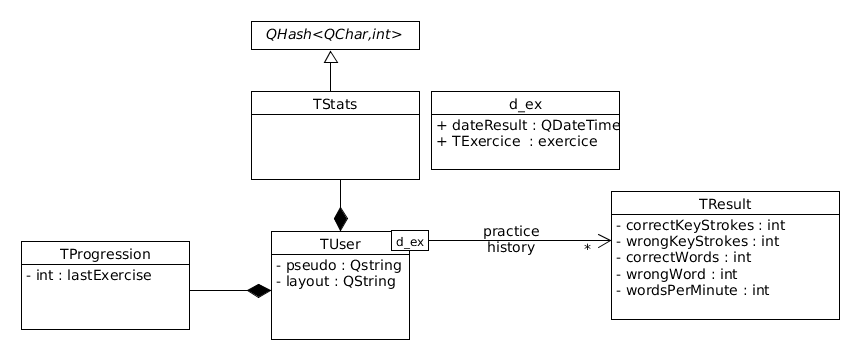
\includegraphics[width=0.7\textwidth]{images/diagram-data.png}
	 \caption{The user's data}
	 \label{diagram-data}
\end{figure}

All the objects represented contains two functions :
\begin{itemize}
	\item One to save the object itself (operator <<)
	\item One to create the object from a save (operator >>)
\end{itemize}

So every time a user was saved, the first function of every object was called, and at the start of the software, all the objects were loaded from the ROM to the RAM by calling the second function. The QSettings class to save the users was voluntary chosen. Since the model is not complex and a very few object are in relationship, the group chose to use QSettings. \\
However, Qt also supports the database operations and provide a support for sqlLite. As said above, there is also a support for XML and JSON. Those last two were not chosen two prevent easy cheating.


\part{System implementation}

\chapter{Building the software}
\section{First prototype}
The first prototype that the group presented to the first demo was giving an idea of the project. It was really fast to build and was containing only one window. On which the user could write down a text. It was a sort of 'proof of concept'. The purpose of this prototype was to demonstrate the main feature of the software and it was also a starting point for the group.\\
The first prototype was containing only two C++ classes. One for the whole window, and one for each row. Even if the prototype was working well, the interface was not very user-friendly and an offset could easily appear when the user was making too many mistakes.
Meaning that even if the prototype was working, a lot of work would be necessary to improve the user interface. \\
This prototype was also a sort of training for the group, it was the first window ever made with Qt. Because the group members didn't know anything about Qt, it was absolutely normal to have such a poor interface.

\section{Second prototype}
The second an actual prototype is a lot more evolved than the first prototype. There are more features, it's working better and it's more user-friendly. Of course, there is some improvements that remains possible.\\
However, the software is ready for production and can be used by anyone who wants to.\\
The second prototype started with a big improvement of the first prototype. The two lines : one for the text, and one for the text-field where the user can type were merged into a single one. So, as the user would type the text, the current character would be displayed in a certain color, the future characters would also be displayed as 'passed'. Therefore, the offset problem was solved. Thanks to the support of HTML in the label with Qt, the task was quite easy.\\
Now that the group had a functional and user-friendly base, they could start to work on the other parts of the project and use this base for differents features.\\
Here are the list of features that were developed on this base, by order of development :
\begin{enumerate}
	\item random-letters typing. Were the user has to type a random set of letters
	\item random-words typing. Were the user has to type real words
	\item text typing. Were the user has to type an existing text (written by great authors such as George Orwell)
	\item improvement. This exercise is using the statistics of the user to know what mistake is the more frequent
\end{enumerate}
All these differents exercise has its own class. But they also all inherit from the same base class to have access to the same resources such as a timer, a play/pause button, and a score a the end.\\
Then the group worked on different aspects of the main program, such as an interactive keyboard, the user's statistics and a homepage where a use can create its account, connect/disconnect.


\chapter{Current state of the software}
The current state of the software is complete. The software is available on \url{github.com} and can be downloaded for Linux or Windows. Anyone with a computer can download the software and start to learn how to type !
Even if the system is working well, the GUI is improvable. However, since the group is not design experts, they did as they could to create a usable software that does not hurt the eyes. And because the software is made up in C++, it's a bit harder than the web to stylize the interface. Even though Qt provides a CSS-like feature to change the style of every elements in a window.


\part{Testing}

\chapter{Unit testing}
Really early in the development of the software, it became obvious that some key features required unit testing.\\
Luckily Qt provides a way to easily and quickly create unit testing. All the tests of the projects are on the 'test' folder.\\
The tests for this projects were created for two main purpose :
\begin{enumerate}
	\item ensure that the feature are working as expected
	\item avoid compiling all the project for a single feature test
\end{enumerate}
Some test requires the GUI some does not. The hard part of the test was not to create them, it was to make the software testable. For example, a lots of features held on randomness. And it is not possible (or silly) to test randomness. This means, the less randomness, the more testable. Or pseudo-random features were testable.\\
Here is an example of a test file :

\begin{lstlisting}
//includes [...]
class TestUtils : public QObject {
    Q_OBJECT
private slots:
    void testSurroundAll();
    void testSurroundAt();
    void testRemoveTags();
    void testAbsolutePosition();
};
\end{lstlisting}
First, the test class must be declared. The whole test can be written in a single .cpp file.\\
To be able to run the test on the class, it must inherit from QObject. Then the Qt test framework will execute the test on all the
private slots.\\
In this case, the HTML helper is tested. Four functions are created to test it.

\begin{lstlisting}
void TestUtils::testAbsolutePosition() {
    QString joel_0 = "joel";
    QString joel_1 = "<p>j</p>oel";
    QString joel_2 = "jo<p>e</p>l";
    QString joel_3 = "joe<p>l</p>";
    QString joel_4 = "<p>j</p>o<b>e</b><u>l</u>";
    QString joel_5 = "<b><u>j</b></u>oel";

    qDebug() << "Get the absolute position of a char in a String";
    QCOMPARE(html::getAbsoluteCharPosition(joel_0, 0), 0);
    QCOMPARE(html::getAbsoluteCharPosition(joel_1, 0), 3);
    QCOMPARE(html::getAbsoluteCharPosition(joel_2, 2), 5);
    QCOMPARE(html::getAbsoluteCharPosition(joel_3, 3), 6);
    QCOMPARE(html::getAbsoluteCharPosition(joel_4, 3), 20);
    QCOMPARE(html::getAbsoluteCharPosition(joel_5, 1), 15);
}

//Other functions...

QTEST_MAIN(TestUtils)
#include "testutils.moc"
\end{lstlisting}
Here is how a function test looks like. As a lot of other test framework, there is the initialization part, the action part and the test part. Qt provides functions as \texttt{QCOMPARE},\texttt{QVERIFY} and others to run the test. To run the test, the file must be compiled and run. In this case, there is no graphics, all is displayed in the console. Here is the output when the entire file is run.

\begin{lstlisting}
********* Start testing of TestUtils *********
Config: Using QtTest library 5.2.1, Qt 5.2.1
PASS   : TestUtils::initTestCase()
QDEBUG : TestUtils::testHTML() Testing HTML 
QDEBUG : TestUtils::testHTML() Adding a single tag 
QDEBUG : TestUtils::testHTML() Adding multiples tags 
QDEBUG : TestUtils::testHTML() Adding attributes 
QDEBUG : TestUtils::testHTML() Remove all the tags 
QDEBUG : TestUtils::testHTML() Remove only the asked tags 
QDEBUG : TestUtils::testHTML() Remove all the tags (no second arguments) 
QDEBUG : TestUtils::testHTML() Get the absolute position of a char in a String 
PASS   : TestUtils::testHTML()
QDEBUG : TestUtils::testFactory() Changing locale for test purpose 
QDEBUG : TestUtils::testFactory() Testing factory (non-random functions) 
QDEBUG : TestUtils::testFactory() ("of", "do", "off", "food") 
QDEBUG : TestUtils::testFactory() ("be") 
QDEBUG : TestUtils::testFactory() ("be", "we", "went", "been", "between", "new", "ten") 
QDEBUG : TestUtils::testFactory() Testing practice generation 
QWARN  : TestUtils::testFactory() Warning : no letters available to generate the practice 
QDEBUG : TestUtils::testFactory() Must contain only real words 
QDEBUG : TestUtils::testFactory() Must contain existing and random words 
QDEBUG : TestUtils::testFactory() Testing that the generation is completely random 
QDEBUG : TestUtils::testFactory() Testing the text generation 
QDEBUG : TestUtils::testFactory() ("into", "a") 
QDEBUG : TestUtils::testFactory() ("into", "one;", "and", "that,", "whilst", "this", "planet", "has", "gone", "cycling", "on", "according", "to", "the", "fixed", "law", "of", "gravity,", "from", "so") 
PASS   : TestUtils::testFactory()
PASS   : TestUtils::cleanupTestCase()
Totals: 4 passed, 0 failed, 0 skipped
********* Finished testing of TestUtils *********
\end{lstlisting}
The series of test is passing, to help the developer identify what part of the test is running, it is possible to output messages.
At the end of the tests, the number of passed, failed an skipped is indicated.

\chapter{GUI testing}
The GUI testing was create to avoid reproducing a big number of steps before being able to realize the real test. It allows the developer to :
\begin{enumerate}
	\item Test only the part wanted of the software
	\item Avoid wasting time compiling the whole software when only a single part of it is necessary.
\end{enumerate}

A GUI testing file is consisting of a really few lines, where the window/widget is created, modified and shown. Then all the developer has to do is to directly use the interface to test what he wants.\\
The group did set-up a lots of these test. Every single dialog has its own test file.

\part{Usability - Users tasks}

\chapter{What can the user do}
The finished software allows the user to do the following tasks:
\begin{itemize}
	\item Start the executable of the software.
	\item Connect to its profile on the homepage of the software.
	\item Create a new user on the homepage.
	\item Delete his profile on the homepage.
	\item Change his settings (alias,keyboard layout, software language)
	\item Select a part of the software were to navigate to
	\item Start a new training on the training page and learn new letters
	\item Unlock the next training exercise if the user was fast enough at the previous one
	\item Start a new practice exercise. The exercise can be one of the following 
	\begin{itemize}
		\item Race : type the most words before the time runs out
		\item Classical : type the given words until the end
		\item Text : type the given text until the end
		\item Improve : type the given words specially chosen from the mistake made during a training
	\end{itemize}
	\item See his statistics at the end of a run :
	\begin{itemize}
		\item Number of words per minute
		\item Number of correct keystrokes
		\item Number of wrong keystrokes
	\end{itemize}
	\item Start the interactive keyboard and see what finger is used to type a certain letter
	\item Disconnect and close the window without losing all his data
\end{itemize}


\chapter{Overall aesthetic}
The software is not beautiful to look but its not ugly either. Because this was the first time the group ever used Qt, the main goal was not to create a fully user-friendly interface. But a usable, interactive and intuitive interface. Moreover, since the interface look-and-fell changes for each OS, it would have been hard to create a unified interface, not matter the OS. The biggest effort in therm of aesthetic were made for the look-and-feel of the exercise/training window. Where the user can instantly understand how the cursor is moving, when the answer given is correct an when it's wrong. This interface will not change, no matter what is the OS. Because all is wittingly chosen :
\begin{itemize}
	\item The color of the font
	\item The size of the font
	\item The font itself (monospace)
\end{itemize}
All the others part of the software will depend on the OS. For example the font of the button will be \textit{Ubuntu} for the Ubuntu OS, but it will be \textit{Verdana} for windows. Same thing for the button. They will look flatter on windows 10 than on ubuntu.


\part{Conclusion and further work}

\chapter{Project result}
In order to determine how successful the project was, it's important to look back at the goals which were set at the beginning of it. These goals are outlined in the project proposal.\\
Here is the list of what these goals were :

\begin{itemize}
	\item Learn how to use Qt framework.
	\item Create a free software with Qt.
	\item Let the source code open and free for all on Github.
	\item Create a software that can teach you how to improve your typing skills.
	\item Allow different keyboard layouts.
	\item Translate this software in different languages.
\end{itemize}

All these requirements has been met except the last one which was to translate the software into different languages.\\
The group succeeded to create an adaptable software to will automatically change its configuration depending on the user's computer. Event if, for now, only two languages are available, anyone can create a file with the most common words of his language and insert it into the software without having to change anything in the code. The same goes for for the texts and the keyboard layouts. Only two languages are available but one can easily type new texts or create a new JSON file for the layout and insert them into the software without having to change anything in the code.\\
Because the software is made for private usage and does not contain any sensible informations, there is no security in place, only a simple login system without password.\\
The software is compiled in release mode en ready for distribution on Windows OS, Ubuntu and Mac OS.


\chapter{Possible improvements}
Here is a list of the possible improvements for the software :
\begin{itemize}
	\item Correct all the memory leaks. Even if the group made all its possible to correct the most of them, some remains and may slow down the software.
	\item Improve the user interface. The minimum was made to make the interface usable. There is a lot of improvement possible.
	\item Create more games to learn the funny way. The software is a bit to formal and not really appropriate for kids.
	\item Allow the user to race with other people (on the same computer or online). Because playing all alone can be boring. When comparing the speed with someone else, this could motivate the user to train more and more to win at these races.
	\item Add statistics. For now, the user has an history of the exercise made, but these are not displayed. This means the user can only see the result of the exercise at the end of it. But then, there is no way for him to know the improvements he made.
	\item Create more practice mode. A strong a usable base was made for the practice exercise, and a lot more game mode can be created in a very few lines. For examples, a mode were at each wrong keystrokes the timer gain a certain number of seconds, this pushes the user to focus on the accuracy rather than the speed.
\end{itemize}


\chapter{Further work}
If the group were to continue developing this software, then there are a few things to aim for.\\
First of all, use Qt a better way. Even if a lot of features of Qt were used, the group may have missed a lots of them. Just for the user interface design for example where only the basic features were used. Qt is really powerful and during this project, the group only had the opportunity to brush the possibilities of Qt. This framework is almost a other language because of its magnitude.\\
A better C++ code would be another aim of the group. The actual code is not perfect and can be improved to be more flexible and more maintainable. Furthermore, improving the C++ quality code would reduce the number of memory leaks of the software. This would improve the speed of the software.\\
The documentation of the project is generated thanks to a program called Doxygen. Only the basics options are enabled on this program. Doxygen allows options that the group did not use and could make the documentation more readable.\\
Lastly, a little website to distribute the software would be a great plus to the software. Since it is only available on github which is mainly for developers, the individuals won't be able to download it easily. The website would give an easy access to anyone who wants to use the software without having to pass by github.\\
